
%\documentclass[a4paper,11pt]{article}
\documentclass{article}

\usepackage[hangul]{kotex}
\usepackage{enumitem}
\usepackage{mathtools}
\usepackage{stmaryrd}
\usepackage{float}
\usepackage{multirow}
\usepackage{array}
\usepackage[margin=1in, bottom=1in]{geometry}

%\usepackage[bitstream-charter]{mathdesign}
%\usepackage[T1]{fontenc}

\setlength{\hoffset}{-25pt}
\addtolength{\textwidth}{50pt}
\setlength{\voffset}{-60pt}
\addtolength{\textheight}{130pt}

\newcommand{\w}[1]{\ensuremath{\textit{#1}}}
\newcommand{\x}{\times}
\newcommand{\rem}{\mtt{\%}}
\newcommand{\rar}{\rightarrow}
\newcommand{\Rar}{\Rightarrow}
\newcommand{\U}{\cup}
\newcommand{\join}{\sqcup}
\newcommand{\ttt}[1]{\texttt{#1}}
\newcommand{\mtt}[1]{\mathtt{#1}}
\newcommand{\bigspace}{\,\,\,\,\,\,\,\,}

\newcommand{\op}[2]{\mtt{#1(}#2\mtt{)}}
\newcommand{\module}[3]{\mtt{#1(}#2\mtt{)(}#3\mtt{)}}
\newcommand{\conc}{\mtt{@}}
\newcommand{\ind}[1]{\mtt{[}#1\mtt{]}}
\newcommand{\indr}[2]{\mtt{[}#1\mtt{:}#2\mtt{]}}
\newcommand{\ifs}[3]{\mtt{if}\,\,#1\,\,\mtt{then}\,\,#2\,\,\mtt{else}\,\,#3}

\newenvironment{prepost}[4]{
  \begin{tabular}{|>{\centering}m{0.4\textwidth}|p{0.6\textwidth}|}
    \hline
    \multicolumn{2}{|l|}{\texttt{#1}} \\ \hline
      \multirow{4}{*}{#2}
     & Require \\ \cline{2-2}
     & #3 \\ \cline{2-2}
     & Guarantees \\ \cline{2-2}
     & #4 \\ \hline
  \end{tabular}
}

\newenvironment{prepostc}[5]{
  \begin{tabular}{|>{\centering}m{0.4\textwidth}|p{0.6\textwidth}|}
    \hline
    \multicolumn{2}{|l|}{\texttt{#1}} \\ \hline
      \multirow{6}{*}{#2}
     & Require \\ \cline{2-2}
     & #3 \\ \cline{2-2}
     & Guarantees \\ \cline{2-2}
     & #4 \\ \cline{2-2}
     & Comment\\ \cline{2-2}
     & #5 \\ \hline
  \end{tabular}
}

\newenvironment{onlyc}[3]{
  \begin{tabular}{|>{\centering}m{0.4\textwidth}|p{0.6\textwidth}|}
    \hline
    \multicolumn{2}{|l|}{\texttt{#1}} \\ \hline
      \multirow{2}{*}{#2}
     & Comment\\ \cline{2-2}
     & #3 \\ \hline
  \end{tabular}
}

\newenvironment{itemizec}{
  \begin{itemize}
}{
  \end{itemize}
  \quad
  \vspace{-1em}
}


\begin{document}

\setlist{nolistsep}
\nointerlineskip
\par\noindent
\setlength{\parindent}{0pt}

\section*{Matmul Layers}
\subsection*{\texttt{torch.nn.Linear}}%{{{
\prepostc{torch.nn.Linear(in, out, bias=True)(x)}{
  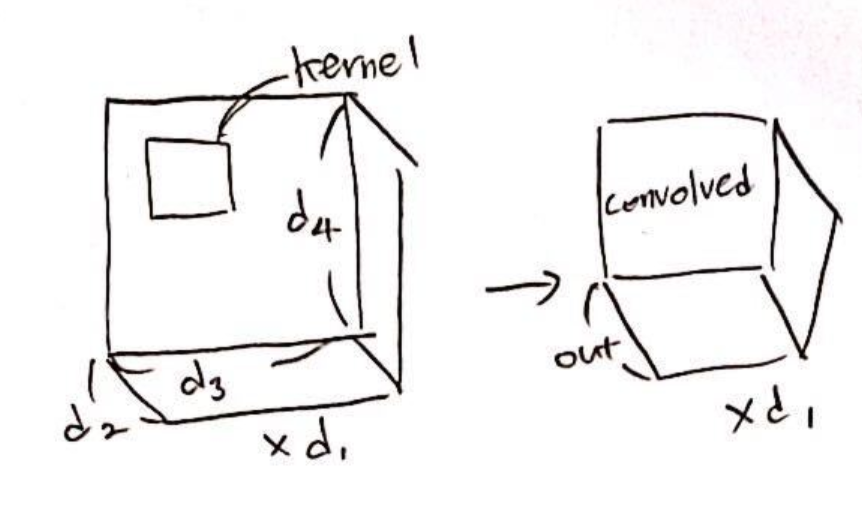
\includegraphics[height=12em]{resources/conv2d.png}
}{
  \begin{itemizec}
    \item $|x| = (d_1, d_2, \dots, d_k)$
    \item $\op{rank}{|x|} \geq 1$
    \item $d_k = in$
  \end{itemizec}
}{
  \begin{itemizec}
    \item $|y| = (d_1, d_2, \dots, d_{k-1}, out)$
  \end{itemizec}
}{
  \begin{itemizec}
    \item $y = x A^T + b$를 계산하는 dense 레이어
    \item $1$차원인 경우에도 잘 작동합니다.
    \item $bias$ 옵션은 출력 shape에 영향을 주지 않습니다.
  \end{itemizec}
}
\begin{align*}
  \frac
  {
    \begin{array}{l}
      \sigma \vdash E \Rar e, c \\
      e' = e[1:k-1] \conc (out) \\
      c' = \{ (\op{rank}{e} \geq 1) \land (d_k = in) \} \\
    \end{array}
  }
  {
    \sigma \vdash \module{Linear}{in, out, bias=True}{E} \Rar e', c \cup c'
  }
\end{align*}%}}}

\section*{Activations}
\subsection*{\texttt{torch.nn.ReLU}, \texttt{torch.nn.ReLU6}, \texttt{torch.relu}, \texttt{torch.nn.functional.relu}}%{{{
\prepostc{torch.nn.ReLU(inplace=True)(x)}{
  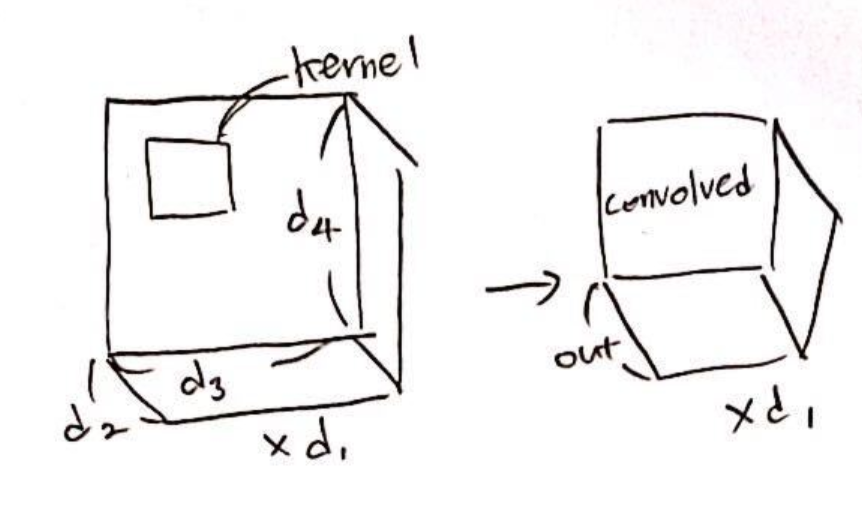
\includegraphics[height=12em]{resources/conv2d.png}
}{
}{
  \begin{itemizec}
    \item $|y| = |x|$ (same shape)
  \end{itemizec}
}{
  \begin{itemizec}
    \item $inplace$ 옵션은 shape에 영향을 주지 않습니다.
    \item \texttt{ReLU6}도 \texttt{ReLU}와 똑같은 방식으로 shape 계산
    \item Bulitins인 \texttt{torch.relu}와 \texttt{torch.nn.functional.relu}는
    같은거
  \end{itemizec}
}
\begin{align*}
  \forall \mtt{ft} \in \{ \mtt{ReLU}, \mtt{ReLU6} \}, \bigspace
  \frac
  {
    \begin{array}{l}
      \sigma \vdash E \Rar e, c
    \end{array}
  }
  {
    \sigma \vdash \module{ft}{inplace=True}{E} \Rar e, c
  }
\end{align*}
\begin{align*}
  \frac
  {
    \begin{array}{l}
      \sigma \vdash E \Rar e, c
    \end{array}
  }
  {
    \sigma \vdash \op{relu}{E, inplace=True} \Rar e, c
  }
\end{align*}%}}}

\section*{Technique}
\subsection*{\texttt{torch.nn.Dropout}, \texttt{torch.dropout}, \texttt{torch.nn.functional.dropout}}%{{{
\prepostc{torch.nn.Dropout(...)(x)}{
  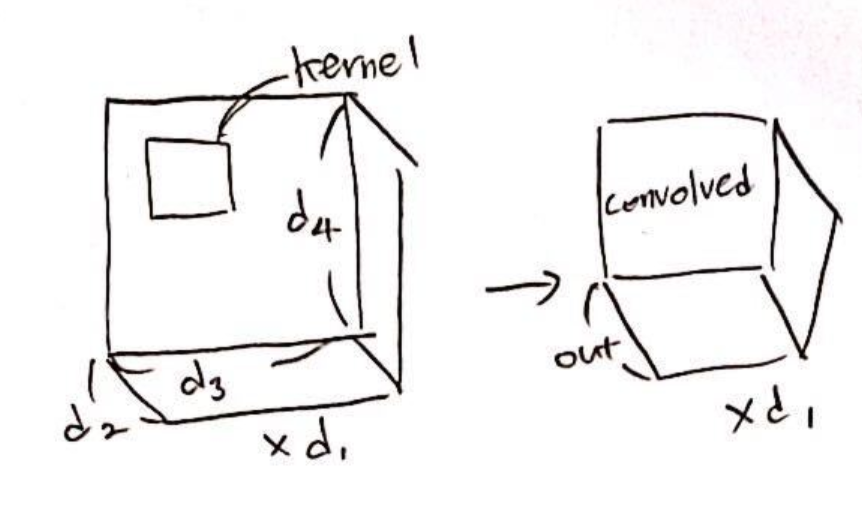
\includegraphics[height=12em]{resources/conv2d.png}
}{
}{
  \begin{itemizec}
    \item $|y| = |x|$ (same shape)
  \end{itemizec}
}{
  \begin{itemizec}
    \item 모든 옵션은 shape에 영향을 주지 않습니다.
    \item Bulitins인 \texttt{torch.dropout}와
    \texttt{torch.nn.functional.dropout}는 서로 역할이 같습니다.
  \end{itemizec}
}
\begin{align*}
  \frac
  {
    \begin{array}{l}
      \sigma \vdash E \Rar e, c
    \end{array}
  }
  {
    \sigma \vdash \module{Dropout}{...}{E} \Rar e, c
  }
\end{align*}
\begin{align*}
  \frac
  {
    \begin{array}{l}
      \sigma \vdash E \Rar e, c
    \end{array}
  }
  {
    \sigma \vdash \op{dropout}{E, ...} \Rar e, c
  }
\end{align*}%}}}

\section*{Wrapper}
\subsection*{\texttt{torch.nn.Sequential}}%{{{
\prepost{torch.nn.Sequential(l1, l2, l3, ..., ln)(x)}{
  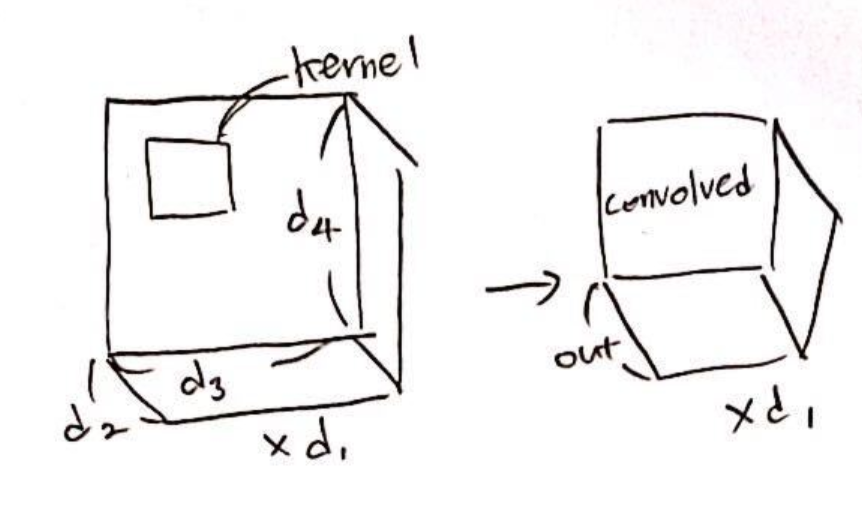
\includegraphics[height=12em]{resources/conv2d.png}
}{
  \begin{itemizec}
    \item 순차적으로 shape이 맞아떨어져야함
  \end{itemizec}
}{
  \begin{itemizec}
    \item $|y| = |l_n \circ l_{n-1} \circ \cdots \circ l_1(x)|$
  \end{itemizec}
}
\begin{align*}
  \frac
  {
    \begin{array}{l}
      \sigma \vdash l_n \circ l_{n-1} \circ \cdots l_1 (E) \Rar e, c
    \end{array}
  }
  {
    \sigma \vdash \module{Sequential}{l_1, l_2, \dots, l_n}{E} \Rar e, c
  }
\end{align*}%}}}

\end{document}
